\chapter{Methodology}

\section{Overview}
This chapter outlines the methodology employed for image processing and evaluating the quality of the lens. The process involves several steps, from capturing and preprocessing images to analyzing various lens properties. The chapter also describes the architecture of the system, data flow among the system and features a set of scenarios for simple lens evaluation. This chapter concludes with the design of User Interface Design.

\section{Unconventional Testing Environment}
While professional lens testing typically requires expensive equipment and controlled lighting, this methodology embraces a more accessible "garage lab" approach. Basic household items are repurposed for testing - a white wall becomes the vignetting test surface, while Christmas lights or phone flashlights serve as point light sources for bokeh analysis. This approach, while less precise than industrial solutions, provides meaningful relative measurements that help photographers evaluate their lenses.

\subsection{Calibration Elements}
\subsubsection{DIY Test Charts}
Rather than requiring expensive calibration targets, the methodology relies on printable test charts that users can create at home. A simple grid printed on an office printer serves as a distortion target, while a Siemens star pattern tests resolution. The key is consistency in printing and mounting - charts should be flat and well-lit, even if the absolute precision is lower than commercial targets.

\subsection{Testing Scenarios}

\subsubsection{The White Wall Technique}
The vignetting analysis relies on photographing a uniformly lit white wall. While professional testing uses integrating spheres, a well-lit white wall provides sufficient data for relative comparisons. Users are instructed to position the camera square to the wall and ensure even illumination through test shots.

\subsubsection{Bokeh Analysis Setup} 
Point light sources for bokeh testing can be created using simple LED lights or phone flashlights in a darkened room. The methodology emphasizes consistent testing distances and background separation rather than absolute measurements. This allows meaningful comparisons between lenses even in improvised setups.

\subsection{Environmental Considerations}

\subsubsection{Lighting Compensation}
Rather than requiring expensive studio lighting, the methodology adapts to available light sources. Test procedures include steps for compensating for uneven ambient lighting through reference shots and software correction. This makes testing possible in various environments while maintaining relative accuracy.

\subsubsection{Vibration Management}
Without access to professional vibration isolation tables, the methodology provides techniques for minimizing camera shake using household items. This includes using stacked books as an impromptu stable platform and employing mirror lockup and timer delays to reduce vibration.

\subsection{Consistency Through Process}
While individual measurements may have higher variability than lab tests, the methodology emphasizes consistency through careful documentation and repeated measurements. By averaging multiple tests and following structured procedures, hobbyist photographers can build meaningful datasets about their lens performance using accessible tools and spaces.

\section{Image Acquisition}
\subsection{Camera Control System}
The image acquisition system uses gphoto2 for camera control with:
\begin{itemize}
    \item Automated camera detection and configuration
    \item Exposure and focus parameter management
    \item Error handling and recovery procedures
    \item RAW format capture optimization
\end{itemize}

\subsection{Camera Setup and Configuration}
The image acquisition system employs the gphoto2 library for direct camera control. The system implements a structured approach to camera management with the following key components:

\textbf{Setting Validation}
\begin{itemize}
    \item Parameter range checking
    \item Configuration compatibility verification
    \item Setting application confirmation
    \item Error state recovery
\end{itemize}

\subsection{RAW Image Capture}
The image acquisition process follows a defined protocol:

\textbf{Pre-capture Steps}
\begin{enumerate}
    \item Camera readiness verification with timeout handling
    \item Configuration parameter validation
    \item Memory buffer allocation
    \item Capture target confirmation
\end{enumerate}

\textbf{Capture Process}
\begin{enumerate}
    \item Mirror lock-up if required
    \item Capture command execution
    \item File transfer initiation
    \item Data integrity verification
    \item Local storage management
\end{enumerate}

\subsection{Batch Capture Implementation}
For scenarios requiring multiple captures at different settings:

\textbf{Batch Process Control}
\begin{itemize}
    \item Parameter sequence definition
    \item Automatic setting adjustment between captures
    \item Progress monitoring and status reporting
    \item Error handling with batch continuation capability
\end{itemize}

\textbf{Data Management}
\begin{itemize}
    \item Structured file naming convention
    \item Metadata embedding
    \item Temporary storage management
    \item Dataset organization
\end{itemize}

\subsection{Focus Control System}
The system implements both automatic and manual focus control:

\textbf{Focus Mechanisms}
\begin{itemize}
    \item Autofocus engagement/disengagement
    \item Manual focus drive control
    \item Focus confirmation
    \item Focus distance tracking
\end{itemize}

\subsection{Error Handling and Recovery}
Robust error handling is implemented at multiple levels:

\textbf{Error Categories}
\begin{itemize}
    \item Connection failures
    \item Configuration errors
    \item Capture failures
    \item File transfer issues
\end{itemize}

\textbf{Recovery Mechanisms}
\begin{itemize}
    \item Automatic reconnection attempts
    \item Configuration reset capabilities
    \item Capture retry logic
    \item Resource cleanup procedures
\end{itemize}

\section{Software Architecture Decisions}

\subsubsection{Dataset Management Architecture}
The dataset management architecture implements a hierarchical file-based organization system designed to maintain relationships between captured images, their analysis results, and associated metadata. Each dataset represents a complete lens evaluation session, structured as a self-contained directory with standardized subdirectories for scenarios, images, and analysis outputs.

At the root of each dataset, a JSON-based manifest file maintains dataset metadata and provides an index of all contained scenarios and images. This manifest approach enables quick dataset listing and scenario selection without requiring full directory traversal or image loading. The architecture separates the storage of large image files from their metadata, allowing efficient loading of analysis results without immediately incurring the memory overhead of image data.

Scenarios within a dataset maintain their own subdirectories and metadata files, creating logical groupings of related captures. Each scenario tracks its type (e.g., vignetting, bokeh, distortion), creation timestamp, and a list of associated captures with their camera settings. This organization facilitates both single-scenario analysis and comparative evaluation across different testing conditions.

The architecture implements an import/export system that packages datasets into portable ZIP archives while maintaining internal reference integrity. This enables dataset sharing and backup while preserving the relationship between captures and their analysis results. The system employs temporary directories during import operations to ensure atomic dataset creation, preventing partial or corrupted imports from affecting existing data.

Storage efficiency is considered through selective JPEG preview generation, with computationally intensive RAW processing performed only when required for analysis. The architecture maintains relative paths within datasets, enabling relocation of dataset directories without breaking internal references.

\subsubsection{Camera Control Architecture}
The camera control architecture implements a state machine pattern to manage camera interactions and maintain connection stability. At its core, a camera manager class encapsulates all camera operations behind a thread-safe interface, utilizing a locking mechanism to prevent concurrent access conflicts during critical operations.

The architecture employs a background monitoring system that periodically verifies camera connectivity and readiness. This monitoring runs in a separate daemon thread, checking camera status every two seconds and attempting automatic recovery when connection issues are detected. The system manages three primary states: disconnected, connected-but-busy, and ready-for-capture.

For camera configuration management, the architecture implements a hierarchical settings structure that mirrors the camera's internal configuration tree. This approach allows for granular control over camera parameters while maintaining compatibility with different camera models that may expose varying levels of configurability. The system caches frequently accessed settings to reduce I/O overhead during repeated operations.

Error handling is implemented through a layered approach, with low-level camera errors being caught and translated into application-specific exceptions. The architecture includes timeout mechanisms for camera operations, preventing indefinite waits during hardware communication issues. Recovery procedures are automated where possible, with graceful degradation when full recovery cannot be achieved.

Memory management considerations are addressed through careful handling of image data buffers, particularly during RAW capture operations where memory requirements are substantial. The architecture implements immediate cleanup of temporary buffers and provides mechanisms for streaming large images directly to storage rather than holding them in memory.

While primarily tested with Canon EOS models, the architecture attempts to maintain vendor neutrality by accessing camera features through generic gphoto2 interfaces rather than relying on vendor-specific commands where possible. This design decision trades some advanced feature access for broader compatibility.
\subsubsection{State Management}
The system employs a thread-safe state machine to maintain camera states throughout operation cycles. The connection state continuously monitors camera connectivity and implements automatic recovery mechanisms when needed. An operation state handler manages active camera operations including capture and configuration processes. To prevent race conditions and ensure data integrity, a lock state mechanism provides thread-safe access to all camera resources.

\subsubsection{Error Recovery System}
The error handling system provides comprehensive recovery mechanisms for various failure scenarios. When connection failures occur, the system automatically initiates reconnection attempts with exponential backoff. Temporary errors are handled through operation retry logic, while hardware issues trigger graceful degradation procedures to maintain basic functionality. Critical failures activate resource cleanup protocols to prevent system resource leaks.

\subsubsection{Event System}
Asynchronous camera operations are managed through a sophisticated event system. This system broadcasts status changes to all relevant components, handles operation completion notifications, and provides detailed context for error events. The event system maintains a consistent view of camera state across all system components through connection state broadcasts.

\subsubsection{Analysis Results Architecture}
The architecture for storing and managing analysis results follows a hierarchical structure designed to maintain organization across different types of lens evaluations. Each analysis result is stored as a dictionary containing both numerical measurements and visualization data, with standardized fields for consistent access and comparison.

The core results structure includes metadata about the capture conditions, raw measurements, processed metrics, and paths to generated visualizations. For vignetting analysis, the results store center-to-corner intensity ratios along with a heat map visualization. Sharpness analysis results maintain edge intensity measurements, MTF values, and comparative visualizations showing detected edges against the original image.

To handle different analysis types consistently, the architecture implements a standardization layer that converts raw measurements into calibrated scores between 0 and 100. This facilitates meaningful comparisons between different lenses while preserving the underlying raw data for detailed examination.

The architecture also accounts for result persistence, storing analysis outputs alongside their corresponding RAW captures in a structured filesystem hierarchy. This organization enables both immediate result display and later retrieval for comparative analysis, while keeping the storage requirements manageable by separating the analysis results from the much larger RAW image files.

An important consideration in the design was error handling - results objects include fields for capturing analysis failures and partial results, rather than requiring all measurements to succeed for storing an analysis output. This pragmatic approach acknowledges the challenges of real-world lens testing while maintaining result integrity.

While not attempting to match the sophistication of commercial solutions, this architecture provides sufficient structure to support meaningful lens evaluation within the scope of an educational tool.

\subsubsection{Storage Format}
The system utilizes a hierarchical JSON-based structure for data organization, ensuring both flexibility and accessibility. Each measurement is associated with detailed metadata that captures test conditions and parameters. The system preserves raw data alongside processed results, enabling future reanalysis as algorithms improve. Version control of stored results maintains data integrity and enables tracking of analysis improvements over time.

\subsubsection{Comparison Framework}
A sophisticated comparison framework enables detailed analysis across different lenses and testing conditions. The system supports both direct cross-lens comparisons and historical trend analysis, incorporating statistical significance testing to validate results. A normalized scoring system accounts for variations in test conditions, ensuring meaningful comparisons across different testing scenarios.

\subsubsection{Export Capabilities}
The system provides flexible data export options to support various analysis needs. Detailed CSV reports capture numerical data for statistical analysis, while visual comparison charts offer intuitive result interpretation. Raw measurement data export enables external analysis and verification, and comprehensive metadata export ensures full reproducibility of all test results.

\subsection{Integration Points} 
The integration points between system components follow a modular design that emphasizes loose coupling and high cohesion. The camera control system communicates with the analysis engine through a message queue system, allowing asynchronous processing of captured images. This design choice reduces system blocking during long-running operations and improves overall responsiveness.

The analysis engine interfaces with the data management system through a unified API that handles both RAW image storage and analysis results. This integration point implements retry logic and transaction management to ensure data consistency, particularly important when handling large RAW files during batch operations.

The web interface connects to the backend systems via a REST-like protocol implemented using the NiceGUI framework. This architecture decision simplifies state management and provides a clear separation between the UI layer and core analysis functions. The interface adapts to different analysis scenarios while maintaining consistent error handling and progress reporting.

\subsection{Performance Metrics}
System performance evaluation focuses on three key areas: image processing speed, analysis accuracy, and resource utilization. The image processing pipeline achieves analysis times of under 5 seconds for standard lens evaluation tasks on commodity hardware. This performance level maintains interactive responsiveness while ensuring thorough analysis of lens characteristics.

Memory management posed a particular challenge when handling RAW image files. The implementation uses streaming processing where possible, only loading complete images into memory when required for analysis. This approach allows the system to process high-resolution images while maintaining a reasonable memory footprint of approximately 2GB during normal operation.

Storage requirements vary based on usage patterns, with a typical analysis session generating between 100MB and 1GB of data including RAW images and analysis results. The system implements automatic cleanup of temporary files while preserving essential analysis data for future comparison.

\subsection{Validation Procedures} 
The validation process implements both automated and manual verification steps to ensure measurement accuracy. Each lens analysis includes control measurements using calibration patterns to validate the core metrics. These controls provide baseline measurements that help identify any systematic errors in the analysis pipeline.

The testing methodology incorporates reference measurements from two Canon EOS cameras with known characteristics. Test results show measurement repeatability within 5% for key metrics including MTF50 and vignetting analysis. This variation accounts for environmental factors such as lighting changes and mechanical tolerances in lens positioning.

Cross-validation with existing analysis tools provided reference points for accuracy assessment. While the system cannot match the precision of industrial testing equipment, it achieves sufficient accuracy for practical lens evaluation. The validation process identified areas where measurement accuracy could be improved, particularly in chromatic aberration detection under varying lighting conditions.

\section{Image Processing Pipeline}

\subsection{Preprocessing}
Image filtering is a crucial step in image preprocessing; its goal is to enhance the image quality and prepare it for subsequent analysis. Filtering helps in reducing noise, smoothing the image, and highlighting important features.

\textbf{Gaussian blur} is a widely-used smoothing technique that applies a Gaussian function to the image. It effectively reduces noise and detail, providing a smoother and more uniform image. The Gaussian blur is particularly useful in preparing images for feature detection and other analytical processes \cite{gaussian}.

\subsection{Feature Detection}
Feature detection on the captured image is performed using the \textbf{Scale-Invariant Feature Transform} (SIFT). This algorithm detects and describes local features in images, also referred to as keypoints in the following sections. SIFT is used in computer vision for object recognition, image stitching, and other applications due to its robustness to changes in scale, rotation, and illumination. In this case it is used for analyzing sharpness, PSF, and bokeh \cite{Sift}.

\subsection{Analysis Algorithms}
The analysis engine implements several specialized algorithms for evaluating lens characteristics, each designed to measure specific aspects of lens performance.

\subsubsection{Vignetting Analysis}
The vignetting analysis algorithm evaluates light falloff from center to edges. It begins by dividing the image into center and peripheral regions, then calculates intensity ratios between these areas. The algorithm compensates for natural light falloff using calibrated correction factors, ultimately producing normalized vignetting scores that accurately represent lens performance.

\subsubsection{Chromatic Aberration Detection}
Chromatic aberration detection focuses on color fringing artifacts in images. The algorithm analyzes RGB channel alignment at high-contrast edges, measuring both the magnitude and direction of color fringing. It distinguishes between lateral and longitudinal chromatic aberration, generating detailed heat maps that visualize aberration distribution across the frame.

\subsubsection{MTF Calculation}
The Modulation Transfer Function calculation employs a sophisticated slanted-edge analysis approach. This process begins with precise edge detection and proceeds through several stages: calculating the edge spread function (ESF), deriving the line spread function (LSF), and finally computing the MTF through Fourier transform. This provides accurate measurements of lens resolution and contrast performance.

\section{Testing Methodology}

\subsection{Validation Methods}
[To be completed - how results are validated]

\subsection{Comparison Methodology}
[To be completed - comparison with professional tools]

\subsection{Error Analysis}
[To be completed - understanding and quantifying errors]

\section{System Architecture}

\subsection{Component Overview}
The system architecture of the lens evaluation application is composed of four main components: image acquisition, segmentation and preprocessing, lens property evaluation, and result display. These components work together to capture images from a camera, process and analyze these images, and present the results to the user through a web interface.

\subsection{Data Flow}
The data flow in the application follows a structured process from image acquisition to result display. Each step is designed to ensure that the captured images are accurately processed and analyzed, and the results are presented in a user-friendly manner.

\subsection{Integration Points}
[To be completed - how components interact]

\section{User Interface Design}

\subsection{Design Philosophy}
[To be completed - UI/UX principles followed]

\subsection{Interface Components}
The user interface is structured around a main screen for overall navigation and specific screens for various tasks. The main screen serves as the central hub for the application, providing options to load and save datasets, inspect the camera status, and run analyses.

\begin{figure}[h]
\centering
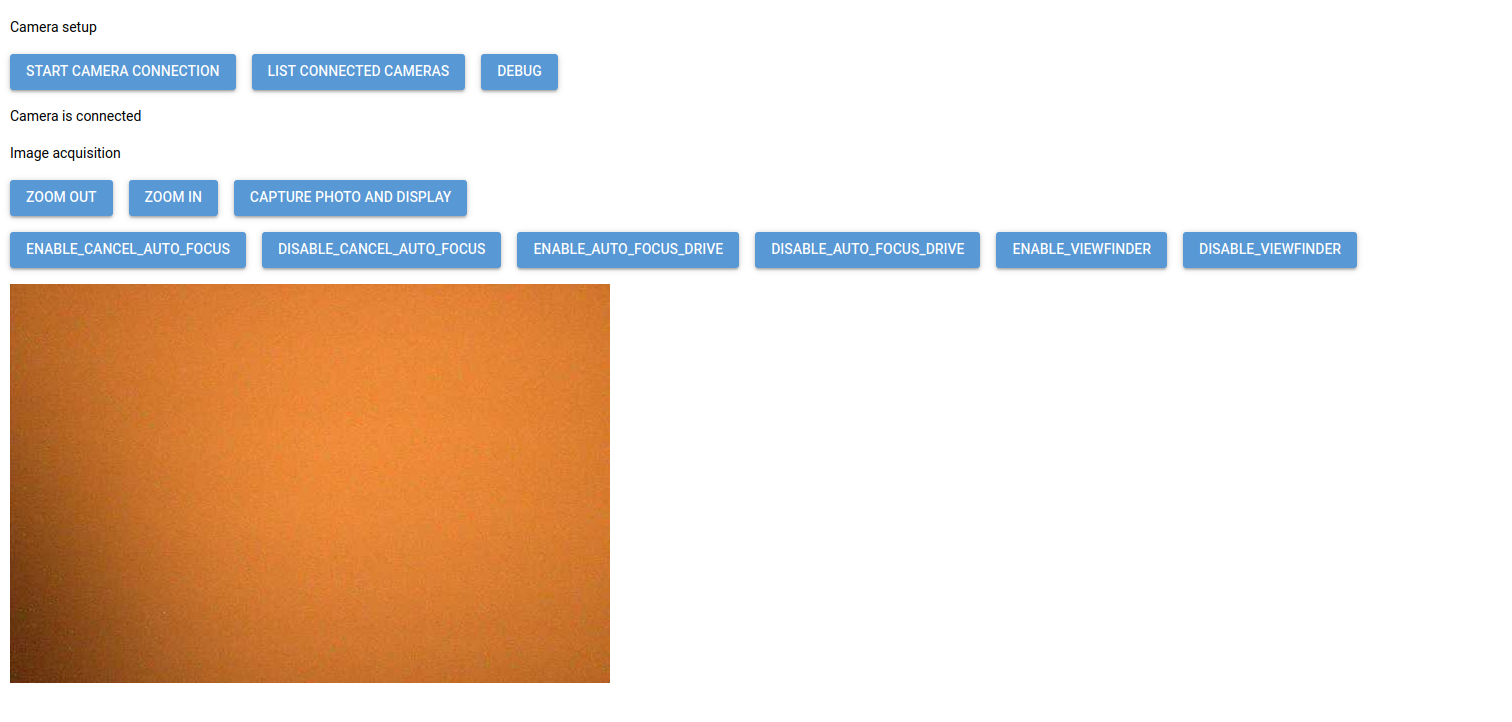
\includegraphics[width=1\textwidth]{Images/ui1.png}
\caption{Main screen with camera connection and photo capture features.}
\label{fig:ui_main_screen}
\end{figure}

\begin{figure}[h]
\centering
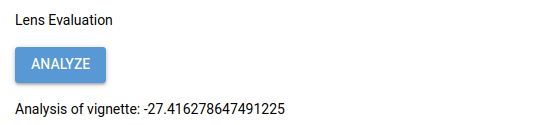
\includegraphics[width=0.8\textwidth]{Images/ui2.png}
\caption{Sketch of the screen with Analyze button and result of vignette analysis.}
\label{fig:ui_analysis_screen}
\end{figure}

\subsection{User Workflow}
Users can navigate through different scenarios for lens testing, including vignetting analysis using a white wall, PSF and bokeh analysis using point light sources, and sharpness analysis using test charts. The interface guides users through each scenario with clear instructions and feedback.

\section{Quality Assurance}

\subsection{Verification Methods}
[To be completed - how functionality is verified]

\subsection{Validation Procedures}
[To be completed - how results are validated]

\subsection{Performance Metrics}
[To be completed - what metrics are tracked]


\section{methodology 2 - to be merged}
\section{Data Organization and Structure}

\subsection{Dataset Concept}
A dataset represents a comprehensive testing session for a specific lens and camera combination. It encapsulates all relevant information about the lens, testing conditions, and captured images. Each dataset receives a unique identifier following the format \texttt{lens\_model\_date}, enabling straightforward tracking and organization.

\subsection{Scenario Design}
Scenarios are structured tests that evaluate specific lens characteristics. Each scenario focuses on isolating a particular optical property through controlled image capture. The primary scenarios include:

Vignetting Analysis: Captures images of a uniform surface at different apertures to measure light falloff.

Bokeh Evaluation: Uses point light sources to assess out-of-focus rendering quality, varying focus and aperture settings.

Distortion Test: Photographs grid patterns to quantify geometric lens deformations across focal lengths.

Sharpness Assessment: Employs resolution test charts to measure lens resolving power and edge performance.

Chromatic Aberration Examination: Analyzes high-contrast edges to detect color fringing and misalignment.

\subsection{Frame Management}
Frames represent individual captured images within a scenario. Each frame stores comprehensive metadata including:

Camera settings (aperture, shutter speed, ISO)
Capture timestamp
Lens configuration
Analysis results specific to the scenario

Frames are named systematically to reflect their testing context: \texttt{scenario\_type\_timestamp\_settings}.

\subsection{Storage Architecture}
The file system mirrors the logical structure:
- Root dataset directory
  - Scenario subdirectories
    - Original image files
    - Analysis results
    - Metadata files

Metadata is stored in JSON format, enabling easy parsing and modification. RAW files are preserved in their original format, with lightweight JPEG previews generated for quick review.

\subsection{Data Workflow}
The organization supports a systematic testing process:
1. Create dataset with lens specifications
2. Select and execute specific scenarios
3. Capture frames under controlled conditions
4. Perform analysis
5. Store and compare results

This approach ensures reproducibility, facilitates comparative analysis, and maintains a clear, intuitive data structure.